%!TEX TS-program = xelatex
%!TEX encoding = UTF-8 Unicode
\documentclass[12pt,a4paper]{article}
\usepackage{geometry} % 設定邊界
\geometry{
  top=1in,
  inner=1in,
  outer=1in,
  bottom=1in,
  headheight=3ex,
  headsep=2ex
}
\usepackage{fontspec} % 允許設定字體
\usepackage{xeCJK} % 引入可以設置中文字型的套件
\setCJKmainfont{LiHei Pro} % 設定中文字型
\setmainfont{Georgia} % 設定英文字型
\setromanfont{Georgia} % 字型
\setmonofont{Courier New}
\linespread{1.2}\selectfont % 行距
\XeTeXlinebreaklocale "zh" % 針對中文自動換行
\XeTeXlinebreakskip = 0pt plus 1pt % 字與字之間加入0pt至1pt的間距,確保左右對整齊
\parindent 0em % 段落縮進
\setlength{\parskip}{20pt} % 段落之間的距離

\title{\huge 資訊安全 Final Project} % 設置標題,使用巨大字體
\author{5105056013 吳嘉偉, 5105056019 廖健智, 5105056029 江青霞} % 設置作者
\date{2017/06/23} % 設置日期,預設值為系統當天的日期。
\usepackage{titling}
\setlength{\droptitle}{-8em} % 將標題移動至頁面的上面
\usepackage{listings}
\usepackage{multicol}
\usepackage{color}
\usepackage{wrapfig} %引入可以在多行架構的文章中插入圖片的套件
\usepackage{graphicx} %package to manage images

\usepackage{hyperref} %引入可以使用超連結的套件
\hypersetup{
    colorlinks=true,
    linkcolor=blue,
    filecolor=magenta,      
    urlcolor=cyan,
}
 
\urlstyle{same}


\begin{document}
\clearpage
\maketitle % 顯示標題,下達這個指令才會把標題印出來。

% 設定多欄式頁面
\begin{multicols}{2}

\section{Introduction}
Many online services let users query large public 
datasets: some examples include restaurant sites, 
product catalogs, stock quotes, and searching for 
directions on maps. In these services, any user can 
query the data, and the datasets themselves are not 
sensitive. However, web services can infer a great 
deal of identifiable and sensitive user information 
from these queries, such as her current location, 
political affiliation, sexual orientation, income, 
etc.
		
\section{Proposed Method}
\subsection{Splinter}
\subsubsection{Architecture}
There are two main principals in Splinter: the user 
and the providers. Each provider hosts a copy of 
the data. Providers can retrieve this data from a 
public repository or mirror site. For a given user 
query, all the providers have to run it on the same 
view of the data. 
  A user splits her query into shares, using the 
Splinter client, and submits each share to a 
different provider. The user can select any 
providers of her choice that host the dataset. The 
providers use their shares to execute the user’s 
query over the cleartext public data, using the 
Splinter provider library. As long as one provider 
is honest (does not collude with others), the 
user’s sensitive information in the original query 
remains private. When the user receives the 
responses from the providers, she combines them to 
obtain the final answer to her original query.

\subsubsection{Security Goals}
The goal of Splinter is to hide sensitive 
parameters in a user's query. Specifically, 
Splinter lets users run parametrized queries, where 
both the parameters and query results are hidden 
from providers.

Splinter supports a subset of the SQL language, 
hides the information represented by the questions 
marks and the query’s results, but the column names 
being selected and filtered are not hidden.
\subsubsection{Threat Model}
Splinter keeps the parameters in the user’s query 
hidden as long as at least one of the user-chosen 
providers does not collude with others. Splinter 
also assumes these providers are honest but 
curious: a provider can observe the inter- actions 
between itself and the client, but Splinter does 
not protect against providers returning incorrect 
results or maliciously modifying the dataset.

It assume that the user communicates with each 
provider through a secure channel (e.g., using 
SSL), and that the user’s Splinter client is 
uncompromised. The cryptographic assumptions are 
standard. They only assume the existence of one-way 
functions in our two-provider implementation. In 
our implementation for multiple providers, the 
security of Paillier encryption is also 
assumed.
\subsection{Function Secret Sharing}
Function Secret Sharing lets a client divide a function f into function shares f1, f2,..., fk so that multiple parties can help evaluate f without learning certain of its parameters.

%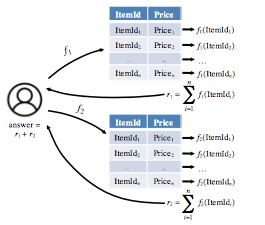
\includegraphics[scale=0.7]{Figure2.png}
%\begin{wrapfigure}{l}{0.9\linewidth}
%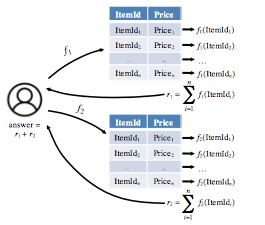
\includegraphics[width=\linewidth]{Figure2.png}
%\caption{This is the Share\LaTeX{} logo}
%\end{wrapfigure}

\section{Case Studies}
\subsection{Restaurant review site}
We implement a restaurant review site using the Yelp academic dataset. The original dataset contains information for local businesses in 10 cities, but we duplicate the dataset 4 times so that it would approximately represent local businesses in 40 cities. We use the following columns in the data to perform many of the queries expressible on Yelp: name, stars, review count, category, neighborhood and location.
For location-based queries, e.g., restaurants within 5 miles of a user’s current location, multiple interval conditions on the longitude and latitude would typically be used. To run these queries faster, we quantize the locations of each restaurant into overlapping hexagons of different radii (e.g., 1, 2 and 5 miles), following the scheme from. We precompute which hexagons each restaurant is in and expose these as additional columns in the data (e.g., hex1mi and hex2mi). This allows the location queries to use ‘=’ predicates instead of intervals.
For this dataset, we present results for the following three queries:
Q1: SELECT COUNT(*) WHERE category="Thai"
Q2: SELECT TOP 10 restaurant
    WHERE category="Mexican" AND
    (hex2mi=1 OR hex2mi=2 OR hex2mi=3)
    ORDER BY stars
Q3: SELECT restaurant, MAX(stars)
    WHERE category="Mexican" OR
    category="Chinese" OR category="Indian"
    OR category="Greek" OR category="Thai"
    OR category="Japanese"
    GROUP BY category
Q1 is a count on the number of Thai restaurants. Q2 re- turns the top 10 Mexican restaurants within a 2 mile radius of a user-specified location by querying three hexagons. We assume that the provider caches the intermediate table for the Top 10 query as described in Section 5.2.3 because it is a common query. Finally, Q3 returns the best rated restaurant from a subset of categories. This requires more communication than other queries because it performs a MAX with many disjoint conditions, as described in Section 5.2.2. Although most queries will probably not have this many disjoint conditions, we test this query to show that Splinter’s protocol for this case is also practical.
\subsection{Flight search}
Implement a flight search service similar to 
Kayak, using a public flight dataset. The 
columns are flight number, origin, destination, 
month, delay, and price. To find a flight, we 
search by origin- destination pairs. 
\subsection{Map routing}
We implement a private map routing service, using real traffic map data from for New York City. However, implementing map routing in Splinter is difficult because the providers can perform only a restricted set of operations. The challenge is to find a shortest path algorithm compatible with Splinter. Fortunately, extensive work has been done to optimize map routing. One algorithm compatible with Splinter is transit node routing (TNR), which has been shown to work well in practice. In TNR, the provider divides up a map into grids, which contain at least one transit node, i.e. a transit node that is part of a "fast" path. There is also a separate table that has the shortest paths between all pairs of transit nodes, which represent a smaller subset of the map. To execute a shortest path query for a given source and destination, the user can use FSS to download the paths in her source and destination grid. She locally finds the shortest path to the source transit node and destination transit node. Finally, she queries the provider for the shortest path between the two transit nodes.
We used the source code from and identified the 1333 transit nodes. We divided the map into 5000 grids, and calculated the shortest path for all transit node pairs. The grid table has 5000 rows representing the edges and nodes in a grid, and the transit node table has about 800,000 rows representing the number of shortest paths for all transit node pairs.

A user issues 2 grid queries and one transit node query. The two grid queries are issued together in one message, so there are a total of 2 network round trips.
and transit node table. One observation is that the multi-party version is slightly faster than the two party version because it is faster at processing the grid query. The two-party version of FSS requires using GMP operations, which is slower than integer operations used in the multi-party version, the two-party version requires much less bandwidth.


\section{Related Work}
\subsection{PIR(Private Information Retrieval ) 
systems}
Splinter is most closely related to systems that 
use Private Information Retrieval(PIR) to query a 
database privately. In PIR, a user queries for the 
ith record in the database, and the database does 
not learn the queried index i or the result. Much 
work has been done on improving PIR protocols. Work 
has also been done to extend PIR to return multiple 
records, but it is computationally expensive. Our 
work is most closely related to the system in, 
which implements a parametrized SQL-like query 
model similar to Splinter using PIR. However, 
because this system uses PIR, it has up to 10⇥ more 
round trips and much higher response times for 
similar queries.

Popcorn is a media delivery service that uses 
PIR to hide user consumption habits from the 
provider and content distributor. However, Popcorn 
is optimized for streaming media databases, like 
Netflix, which have a small number (about 8000) of 
large records.
The systems above have a weaker security model: all
the providers need to be honest. Splinter only 
requires one honest provider, and it is more 
practical because it extends Function Secret 
Sharing (FSS), which lets it execute 
complex operations such as sums in one round trip 
instead of only extracting one data record at a 
time.
\subsection{Garbled circuits}
Systems such as Embark, BlindBox, and 
private shortest path computation systems 
use garbled circuits to perform private 
computation on a single untrusted server. Even with 
improvements in practicality, these techniques 
still have high computation and bandwidth costs for 
queries on large datasets because a new garbled 
circuit has to be generated for each query. 
(Reusable garbled circuits are not yet 
practical.) For example, the recent map routing 
system by Wu et al. uses garbled circuits and 
has 100⇥ higher response time and 10⇥ higher
bandwidth cost than Splinter.
\subsection{Encrypted data systems}
Systems that compute on encrypted data, such as CryptDB, Mylar, SPORC, Depot , and SUNDR, all try to protect private data against a server compromise, which is a different problem than what Splinter tries to solve. CryptDB is most similar to Splinter because it allows for SQL-like queries over encrypted data. However, all these systems protect against a single, potentially compromised server where the user is storing data privately, but they do not hide data access patterns. In contrast, Splinter hides data access patterns and a user’s query parameters but is only designed to operate on a public dataset that is hosted at multiple providers.
\subsection{ORAM(Oblivious RAM) systems}
Splinter is also related to systems that use Oblivious RAM. ORAM allows a user to read and write data on an untrusted server without revealing her data access patterns to the server. However, ORAM cannot be easily applied into the Splinter setting. One main requirement of ORAM is that the user can only read data that she has written. In Splinter, the provider hosts a public dataset, not created by any specific user, and many users need to access the same dataset.
\section{Experimental Result}
Can Splinter be used practically for real applications?  

Built and evaluated clones of three applications on Splinter: restaurant reviews, flight data, and map routing, using real datasets.
Can support realistic applications including the search features of Yelp and flight search sites, and data structures required for map routing.
Achieves end-to-end latencies below 1.6 sec for queries in these applications on realistic data.
Use up to 10x fewer round trips than prior systems and have lower response times. 
 
\section{Implementation} 
\subsection{BinaryTree}
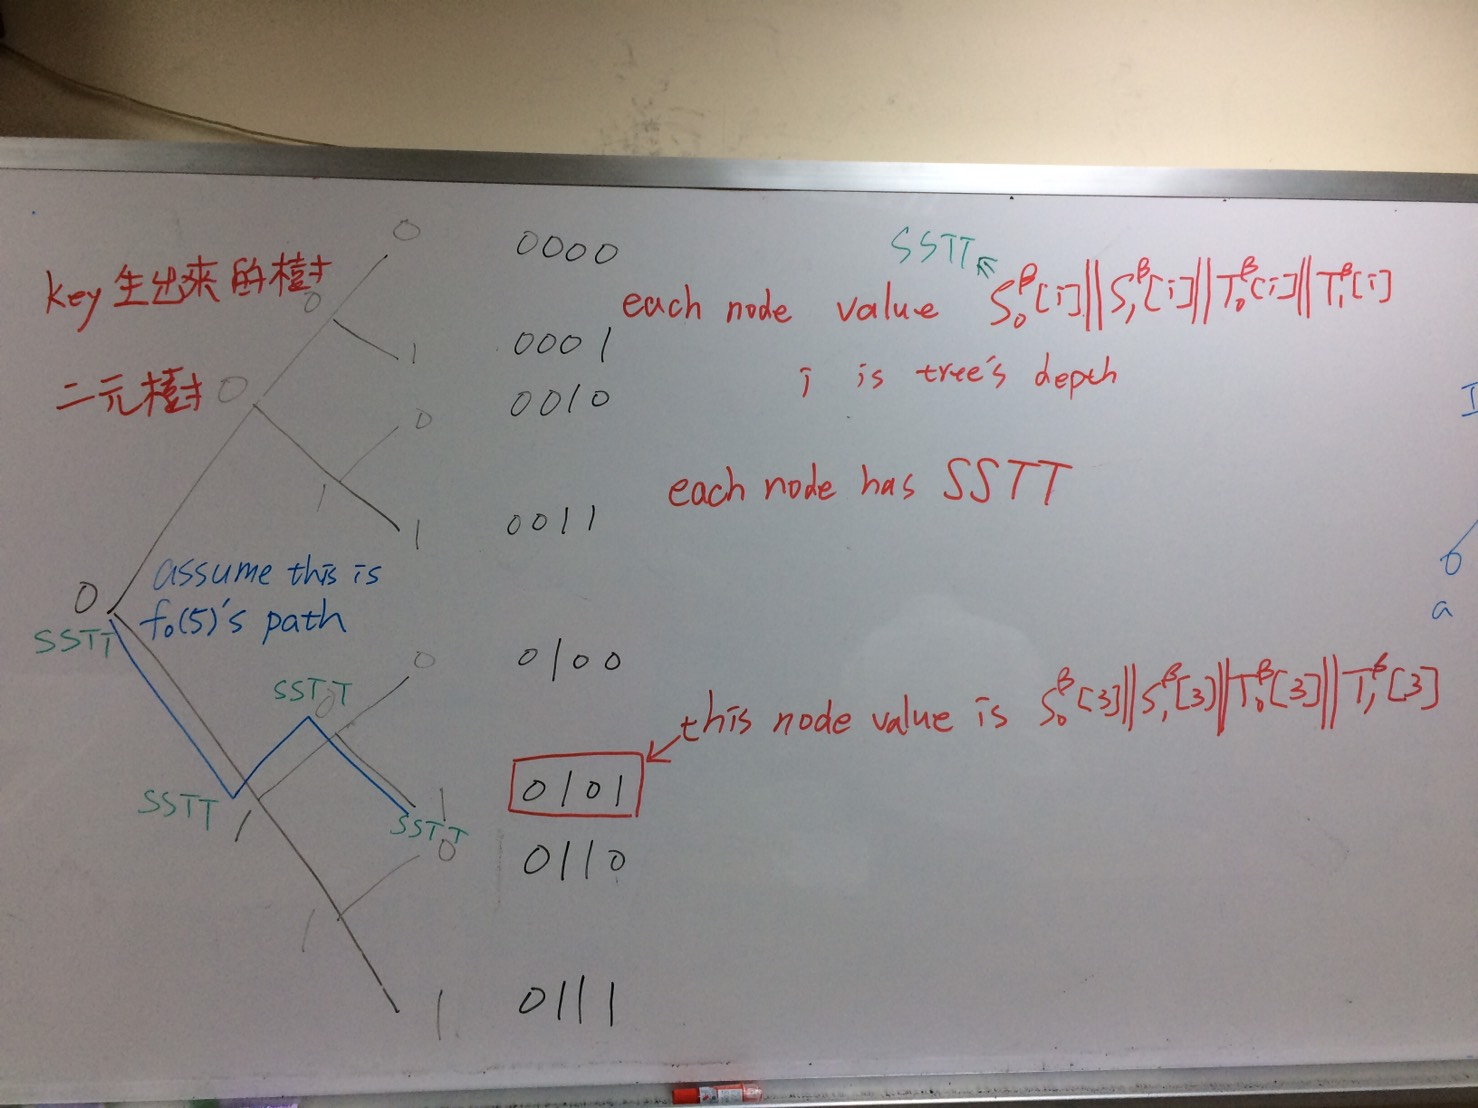
\includegraphics[scale=0.15]{BinaryTree.jpg}
\subsection{HowUserGetInfo}
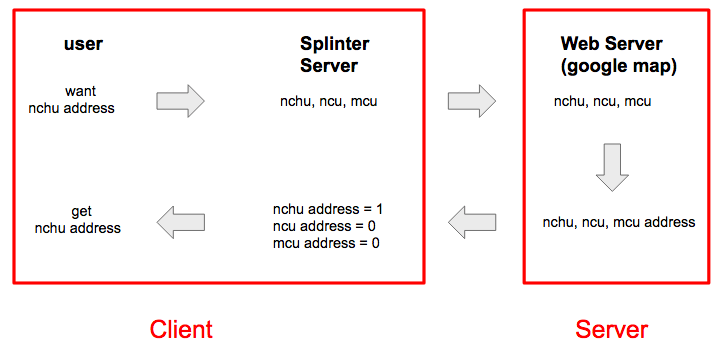
\includegraphics[scale=0.27]{HowUserGetInfo.png}
\subsection{程式截圖說明}
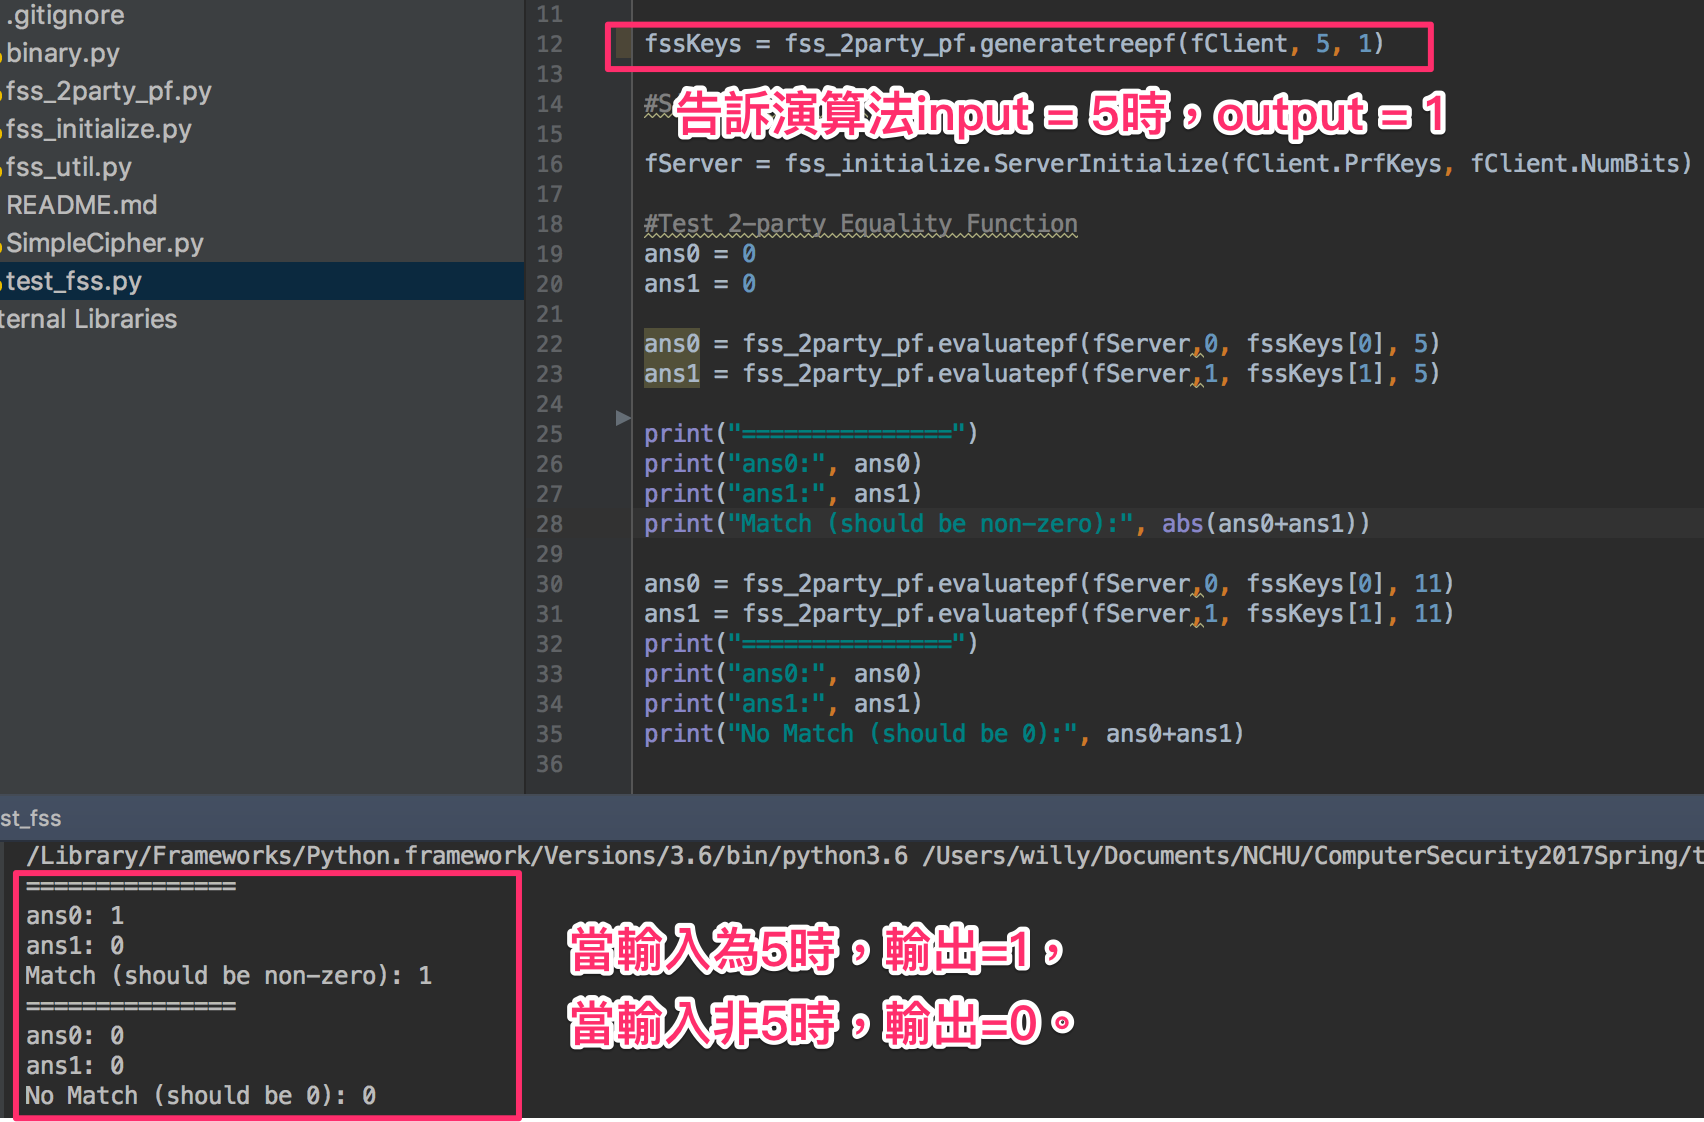
\includegraphics[scale=0.25]{程式截圖說明.png}
\href{https://github.com/WillyWu0201/ComputerSecurity2017Spring}{Source code 連結請點我}

\section{Conclusion}
Splinter is a new private query system that protects sensitive parameters in SQL-like queries while scaling to realistic applications. Splinter uses and extends a recent cryptography primitive, Function Secret Sharing (FSS), allowing it to achieve up to an order of magnitude better performance compared to previous private query systems. [1] Develop protocols to execute complex queries with low computation and bandwidth. As a proof of concept, it has evaluated Splinter with three sample applications—a Yelp clone, map routing, and flight search—and showed that Splinter has low response times from 50 ms to 1.6 seconds with low hosting costs.

\section{Reference}
[1] Splinter: Practical Private Queries on Public 
Data Frank Wang, Catherine Yun, Shafi Goldwasser, 
Vinod Vaikuntanathan, Matei Zaharia† MIT CSAIL, 
†Stanford InfoLab

[2] E. Boyle, N. Gilboa, and Y. Ishai. Function 
secret sharing. In Proceedings of the 34th Annual 
International Confer- ence on the Theory and 
Applications of Cryptographic Techniques 
(EUROCRYPT), pages 337–367. Sofia, Bul- garia, Apr. 
2015.

[3] N. Gilboa and Y. Ishai. Distributed point 
functions and their applications. In Proceedings of 
the 33rd Annual International Conference on the 
Theory and Applications of Cryptographic Techniques 
(EUROCRYPT), pages 640– 658. Copenhagen, Denmark, 
May 2014.
\end{multicols}
\end{document}